%!TEX root = 0.tex

\section{Utool in Practice} \label{sec:practice}

We conclude this manual with some examples for using Utool in
practice.

\subsection{Some practical tips} \label{sec:practice-some-practical-tips}

\begin{enumerate}
\item \textit{Running Utool in server mode.} Whenever you want to
process a large number of USRs in batch mode, you should seriously
consider running Utool in server mode by invoking the \verb?server?
command. This will save the considerable startup time for new Java
processes, and allow the Java virtual machine to just-in-time compile
the bytecode for further efficiency.

\item \textit{Running Java in server mode.} The Sun implementation of
the Java VM can run in either ``client'' or ``server'' mode. The
client mode is the default, but if you have a long-running process,
the server mode can be significantly more efficient because it invests
more time into just-in-time compilation and optimisations.

For optimum performance of Utool, we recommend that you run the JVM in
server mode by calling it as follows:
\begin{verbatim}
$ java -server -jar Utool.jar ...
\end{verbatim}
%$

Because of the increased time for startup and compilation, this works
best if you also run Utool in server mode and send it commands via a
socket. If you do, you can encourage the JVM to JIT-compile the solver by passing the \verb?--warmup? option to the server.

%\begin{figure}
%\begin{center}
%\todo{runtimes for solving chains using server mode and client mode}
%\end{center}
%\caption{Runtimes for the command \texttt{solve -n -s -I chain
%<length>}, running the Java VM in client and server
%mode. \label{fig:chains-server-client}}
%\end{figure}


\item \textit{Memory consumption.} The chart that Utool computes for
large USRs can grow to eat up quite a bit of your memory. If it grows
larger than the heap limit of the Java VM, Java will throw an
\verb?OutOfMemoryError? and terminate the process. For most USRs that
you will encounter in practice (including almost all USRs in the HPSG
treebanks), the default limit of 256 MB will be sufficient. However,
for those cases where more memory is needed (e.g.\
\verb?rondane-650.mrs.pl? in the examples directory, which has about
$2 \cdot 10^{12}$ solved forms), you can allow Java to use more heap
space by calling it with the \verb?-Xmx512m? option.

\item \textit{Character encodings.} Utool displays characters using the default
character encoding of the Java process. On most Unix-based systems (Linux and some versions of MacOS), Java will take its character encoding from the current locale, which you can set by changing the environment variable \verb?LANG? (see also \verb?man locale?). If this is not possible on your system, you can also change Java's character encoding directly by setting the \verb?file.encoding? property.

For instance, say that the default character encoding of your operating system is UTF-8, but you want to use Utool to display an USR that uses German umlauts encoded in Latin-1 (aka ISO-8859-1). You could then either change the locale using the environment variable, like so:

\begin{verbatim}
$ LANG=de_DE.ISO8859-1 utool display some-usr
\end{verbatim}

Alternatively, you could pass the character encoding directly to Java as follows:

\begin{verbatim}
$ java -Dfile.encoding=ISO-8859-1 -jar Utool.jar ...
\end{verbatim}

Note that character encodings are only an issue if you want to display
underspecified representations. If you want to solve an USR, or convert it
into other formalisms, then Utool produces outputs based on the same encoding as
the input.

Some users have reported problems with displaying USRs that contain Chinese characters. This is theoretically no problem, but the practice can be a little tricky. We refer you to the online literature on the topic of using Chinese characters in Java, but here are two ideas to get you started on troubleshooting: (a) Remember to inform Java of the character encoding you use, and (b) you must have fonts that can display Chinese characters and that can be used by Swing, and Java must be able to find these fonts.


\item \textit{XML character entities.} The Utool Server takes commands
as well-formed XML strings, so it expects you to encode special
characters in the USR as XML character entities. You are probably
familiar with having to replace the \"\ character by \verb?&quot;?
etc., and performing the inverse replacement when decoding the
server's responses.

A lesser known aspect of this, however, is that XML parsers will
ignore whitespace within attribute values according to the XML
specification. In particular, you may use newline characters within a
USR, but these characters will be ignored by the parser. If the
concrete syntax of an input codec requires that there are newlines
(e.g.\ to terminate a comment line in the domcon-oz codec), you must
encode this newline character as the character entity \verb?&#xA;?.
\end{enumerate}




\subsection{Writing your own client for the Utool Server}
\label{sec:practice-client}

It often makes sense to run Utool in server mode. In these cases, you
will probably want to implement a client in your own application that
communicates with the server. This is documented in
Section~\ref{sec:operations-server}, but here we give you the source
code of a minimal client written in Perl. This script assumes that a
Utool Server is running on the local machine on the standard port
2802. It will read a USR in \verb?domcon-oz? format from standard
input or a file and send it to the server as the argument of a
\verb?solve? command. It will then wait for an answer from the server
(i.e., a list of solved forms in \verb?term-oz? format) and print it
to standard out.

\begin{verbatim}
use IO::Socket;

# read a dominance constraint
$message = join('', <>);

# open connection
$socket = IO::Socket::INET->new("localhost:2802") or die $!;

# and send it to the server
print $socket <<EOF;
<utool cmd='solve' output-codec='term-oz'>
  <usr codec='domcon-oz' string='$message'/>
</utool>
EOF

# shutdown output side of the socket
$socket->shutdown(1);

# print the answer 
while (<$socket>) { print }
\end{verbatim}
%$

The key point here is that the client shuts down the side of the
socket that is used to send data from the client to the server. This
tells the server that the input is now complete and it should start
processing it.

An extended version of this script (also in Perl) is part of the
standard Utool distribution and can be found in the directory
\url{tools/client}. 




\subsection{Integration with the LKB Workbench}
\label{sec:integration-lkb}


Utool can be used as a drop-in replacement for the MRS solver built
into the LKB grammar development system \cite{Copestake:LKB-Book},
which is freely available at \url{http://www.delph-in.net/lkb}. This means that users of the
LKB now have easy access to our solver, which is considerably faster
than the original MRS solver. The integration between LKB and Utool is
achieved via two Lisp source files that we distribute in the directory
\url{tools/lkb}.

If you load the file \verb|lkb-utool.lisp| into the Lisp console
of a running LKB system, the internal MRS solver is replaced by
Utool. Technically, this file defines a function that sends the MRS
(in \verb?mrs-prolog? syntax) to a Utool Server running on the local
machine on port 2802. It will then receive the solved forms from the
server, in \verb?plugging-lkb? syntax, and pass them back to LKB.


\begin{figure}
\begin{center}
%HEVEA \imgsrc{lkb-integration.png}
%HEVEA \begin{latexonly}
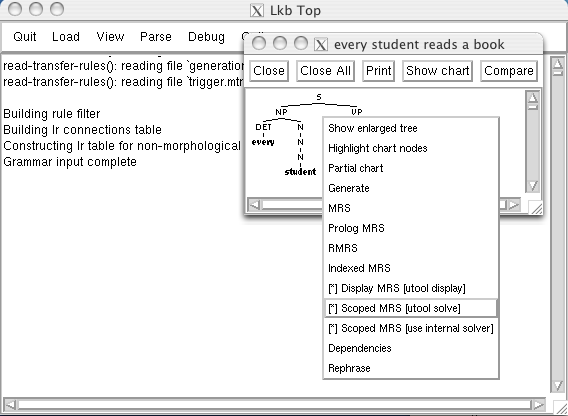
\includegraphics[width=0.8 \textwidth]{lkb-integration}
%HEVEA \end{latexonly}
\end{center}
\caption{Calling Utool from an LKB context menu.
\label{fig:lkb-integration}}
\end{figure}


Alternatively, if you load the file \verb|lkb-utool-menu.lisp|
into the Lisp console, two new commands are added to the context menu
for parse trees (see Fig.~\ref{fig:lkb-integration}). The command
``Scoped MRS (utool solve)'' calls Utool to compute all scopings of
the MRS for this parse tree, in the same way as just described. On the
other hand, the ``Display MRS'' command will ask the Utool Server to
perform a \verb?display? command for the given MRS. You can then solve
and further manipulate the USR from the GUI. As before, these commands
also make the assumption that a Utool Server is running on the local
machine, port 2802.

If your Utool server is running anywhere that's not \verb?localhost:2802?, you can change the host and/or port by setting the variables \verb?utool::*utool-host*? and \verb?utool::*utool-port*? to the values you want in the Lisp console.

One thing to keep in mind when using LKB together with Utool is that LKB seems to use the Latin-1 character encoding when sending USRs over the socket. It would be nice if LKB could be made to send UTF-8, but we haven't managed to figure out how this is done. However, you can always make Utool expect the Latin-1 character encoding, as described in Section~\ref{sec:practice-some-practical-tips}.






\subsection{Extracting USRs from a HPSG treebank}
\label{sec:treebank}

The English Resource Grammar (ERG; \citeNP{Copestake&Flickinger:LKB})
is distributed together with a collection of hand-annotated corpora that contains for each sentence from the corpus
the preferred syntactic analysis and  a corresponding
underspecified semantic representation based upon MRS. These corpora are extremely
valuable resources because corpora with deep semantic information are
so very rare, and we have occasionally used them in experiments
\cite{FucKolNieTha04,FliKolTha05}.

In order to use the MRS structures in these treebanks from within
Utool, it is necessary to extract them from the treebank and save them
in individual files. This can be done by using the script
\verb|extract-gold.lisp|, which can be found in the directory
\url{tools/lkb} in the Utool jar file. Proceed as follows:

\begin{enumerate}
\item Start the LKB system.
\item Locate the treebank file on your filesystem. Here we will assume
that we are working with the Rondane treebank, which is located in
\url{erg/gold/rondane} under the main ERG directory. The \verb|rondane| directory contains a file \verb|result.gz|, which contains the actual annotations and has to be unzipped first.
%You may
%have to unzip the file \verb?result.gz? that comes with the original
%ERG distribution first.
\item Run the following commands in the LKB's Lisp console:
\begin{verbatim}
(load "extract-gold")
(utool::extract-prolog "erg/gold/rondane/result" "target-directory")
\end{verbatim}
You need to replace \verb?target-directory? with the name of the
directory in which you want the individual MRSs stored. This will
create a number of files with the extension \verb?.mrs.pl?, one for
each sentence in the treebank. These files are suitable for reading
with the \verb?mrs-prolog? input codec.
\item If you want MRSs in XML format instead, call
\verb?utool::extract-xml? rather than
\verb?utool::extract-prolog?. The arguments of both calls are the
same. 
\item If you pass the additional argument \verb?:solve t? to the
\verb?extract-prolog? call, the MRS constraint solver is applied to
each MRS expression, and the number of fully scoped MRS expressions is
stored in a file \verb|log| in the target directory. This can be
useful to compare the results of the MRS solver and Utool, but can
take quite a while.
\end{enumerate}

The \verb?extract? functions will work with the treebanks that are
distributed together with the ERG under the \verb|erg/gold| directory,
but they will not work directly with the Redwoods corpus
\cite{Oepen&al:Redwoods}, which is distributed separately and uses a
 different internal format. See e.g.
\url{http://wiki.delph-in.net/moin/RedwoodsTop} for more information
about the Redwoods corpus, and how MRS structures can be extracted.

%\todo{This is not very clear yet:
%\begin{itemize}
%\item What corpora exactly can we convert with the tool in the
%distribution?  Only Rondane, or does JH work too? What do I have to do
%in order to get these corpora? 
%\item What do I have to do to extract the MRSs in the Redwoods corpus?
%Where do I get Redwoods? Why are Rondane etc.\ called
%``Redwoods-style'' if their internal formats are not compatible?
%\end{itemize}
%}



\subsection{Benchmarks}

Utool is the fastest solver for underspecified descriptions in the
formalisms of dominance constraints, dominance graphs, Hole Semantics,
and MRS that exists today. This is supported by theoretical complexity
results
\cite{Althaus-J.Algo.,bodirsky-weakly-normal-constraints,KolTha05b},
and we have previously claimed practical efficiency in various
publications.

We will now sketch how such claims of practical efficiency can be
substantiated. In doing so, we will also establish the fact that the
Java implementation of Utool is not slower than the earlier C++
implementations of Utool under Linux and Windows, and is in fact a
little faster on Windows. We will not report detailed results for MacOS, but the situation is roughly that Java on PowerPC Macs seems to be very slow, but the performance on Intel Macs seems to be comparable with the other platforms on the same processor.



\begin{figure}
%HEVEA \begin{latexonly}
\centering
\begin{tabular}{cc}
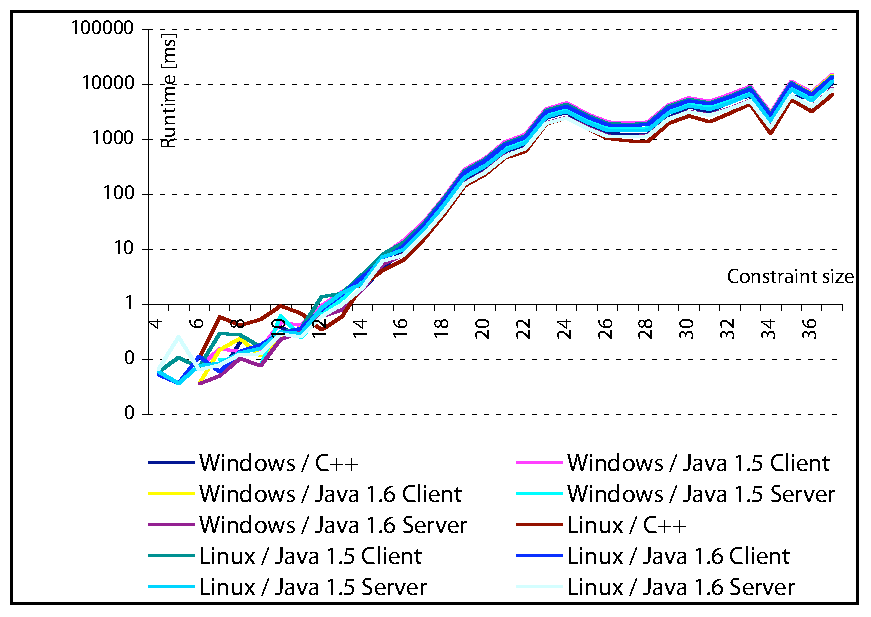
\includegraphics[width=0.48\textwidth]{jh-extraction-mean.pdf}
&
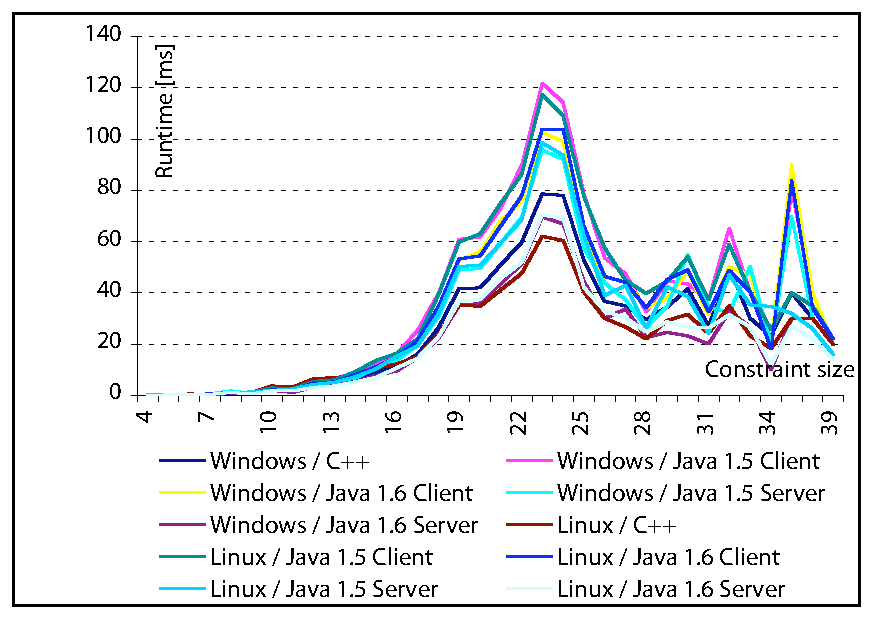
\includegraphics[width=0.48\textwidth]{jh-chart-mean.pdf}
\end{tabular}
%HEVEA \end{latexonly}
%HEVEA \imgsrc{jh-extraction-mean.png}
%HEVEA \imgsrc{jh-chart-mean.png}
\caption{Runtimes for the commands \texttt{solvable} (left) and
\texttt{solve -n} (right) of Utool 2.0.1 (C++) and 3.0 (Java) on
Windows and Linux. \label{fig:runtimes}}
\end{figure}

As our benchmark example, we chose the Jotenheimen corpus, which like
the Rondane corpus (cf. Section \ref{sec:treebank} above) is
distributed together with the English Resource Grammar. The corpus
contains analyses for 5135 sentences together with corresponding
semantic representations based upon MRS. We extracted the MRS
structures as described in Section~\ref{sec:treebank} above and
translated them into dominance graphs. Of the 5135 MRS structures in
the corpus, 441 could not be translated, so we base the evaluation on
a dataset of 4694 dominance graphs.

Then we ran the commands
\verb?utool solvable? (measuring how long it takes to compute the
chart and count all solved forms) and \verb?utool solve -n? (measuring
how long it takes to compute the chart and then extract all solved
forms, without actually encoding or displaying them) on all dominance graphs with at most one million solved forms. We did this
using both Utool 2.0.1 (the last C++ version) and Utool 3.0 (the first
Java version) on all sentences. We ran Utool 3.0 in server mode (using
\verb?utool server?) to eliminate the overhead for starting up the
JVM.

We performed the benchmarks using a machine with a Pentium M processor
at 1.6 GHz, both on Windows XP Professional and on Linux 2.6.10. Utool
2.0.1 was compiled with Gnu C++ 4.0 under Linux and with the C++
compiler from the Microsoft Visual C++ Toolkit 2003. We ran Utool 3.0
both using Java SE 5.0 and using a beta version of Java SE 6.0; in
both cases, we ran the JVM both in client and in server mode (with the
\verb?-server? JVM flag).

The results of these benchmarks are shown in
Fig.~\ref{fig:runtimes}. Both charts plot the size of the
underspecified description (number of fragments in the dominance
graph) on the X axis and the mean runtime for USRs of this size on the
Y axis. Notice that the Y axis is logarithmic in the left-hand picture.
Looking at the
charts, we can make the following observations:
\begin{itemize}
\item The mean time for computing a chart is dramatically lower than
the time for enumerating all solved forms. This is unsurprising, as
the number of solved forms of a graph is typically much higher (and
grows much faster with the graph size) than the number of splits in
its chart (Fig.~\ref{fig:chart-vs-solutions}).
\item Running Java in server mode is generally much faster than
running it in client mode.
\item Even the beta version of Java 6.0 is noticeably more efficient
than Java 5.0.
\item The difference in performance between Utool 2.0.1 and Utool 3.0
running on Java 6.0 in server mode is negligible under Linux. Under
Windows, the Java version is more efficient (although it is
conceivable that the Visual C++ compiler supports optimisations that
we weren't aware of).
\end{itemize}



\begin{figure}
%HEVEA \begin{latexonly}
\centering
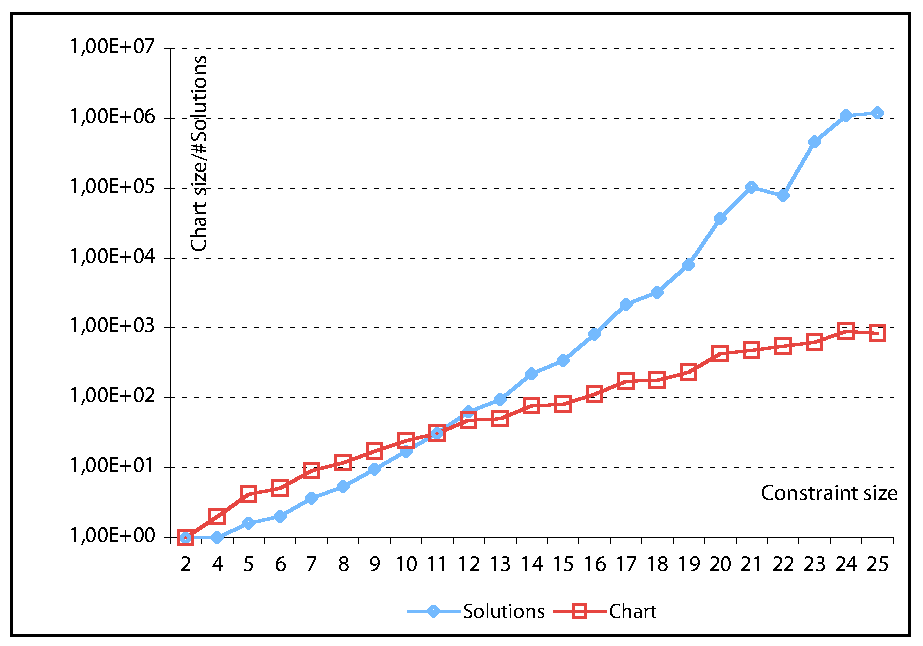
\includegraphics[width=10cm]{chart-vs-solutions.pdf}
%HEVEA \end{latexonly}
%HEVEA \imgsrc{chart-vs-solutions.png}
\caption{The size of the chart as compared to the number of solved
forms described by the chart, for all dominance graphs in the
Jotenheimen corpus with up to 25 fragments. \label{fig:chart-vs-solutions}}

\end{figure}






%%% Local Variables: 
%%% mode: latex
%%% TeX-master: "0"
%%% TeX-command-default: "LaTeX"
%%% End: 
